 \documentclass{article}
\usepackage[utf8]{inputenc}
\usepackage[a4paper, total={7in, 10in}]{geometry}
\usepackage{braket}
\usepackage{xcolor}
\usepackage{amsmath}
\usepackage{amssymb}
\usepackage{amsfonts}
\usepackage{graphicx}
\usepackage{svg}
\usepackage{float}
\usepackage{tikz}
\usepackage[ruled,vlined]{algorithm2e}
\usepackage{multicol}
\usepackage[backend=biber,style=alphabetic,sorting=ynt]{biblatex}
\usepackage{xcolor}
%\addbibresource{sample.bib} %Import the bibliography file

\newcommand{\commentt}[1]{\textcolor{blue}{ \textbf{[COMMENT]} #1}}
\newcommand{\ctt}[1]{\commentt{#1}}
\newcommand{\prb}[1]{ \mathbf{Pr} \left[ {#1} \right]}
\newcommand{\onotation}[1]{\(\mathcal{O} \left( {#1}  \right) \)}
\newcommand{\ona}[1]{\onotation{#1}}
\newcommand{\PSI}{{\ket{\psi}}}
\newcommand{\LESn}{\ket{\psi_n}}
\newcommand{\LESa}{\ket{\phi_n}}
\newcommand{\LESs}{\frac{1}{\sqrt{n}}\sum_{i}{\ket{\left(0^{i}10^{n-i}\right)^{n}}}}
\newcommand{\Hn}{\mathcal{H}_{n}}
\newcommand{\Ep}{\frac{1}{\sqrt{2^n}}\sum^{2^n}_{x}{ \ket{xx}}}
\newcommand{\HON}{\ket{\psi_{\text{honest}}}}
\newcommand{\Lemma}{\paragraph{Lemma.}}


\setlength{\columnsep}{0.6cm}

\newcommand{\Gz}{ G_{z}^{\delta} } 

\begin{document}

\title{Quantum LTC With Positive Rate}
\author{David Ponarovsky}
\maketitle
\begin{multicols*}{2}
\newcommand{ \Hw }{ \delta\Delta -\Delta^{\frac{1}{2}-\varepsilon}/\delta  }
	\newcommand{ \Nw }{ \Delta^{\frac{3}{2}-\varepsilon}} 
	  \newcommand{ \Gu } { \Gamma^{\cup} }
	  \newcommand{ \Guq } { \Gamma^{\cup, \square} }

    	\newcommand{ \Gsa } {\Gamma_{\square_{1}} }
	\newcommand{ \Gsb } {\Gamma_{\square_{2}} }
        \newcommand{ \Aa } { C_{A_{1}}}  
	\newcommand{ \Ab } { C_{A_{2}}}
	\newcommand{ \Ac } { C_{A_{3}}}
	\newcommand{ \Aab } { \Aa \otimes \Ab } 
	\newcommand{ \Aac } { \Aa \otimes \Ac }
	\newcommand{ \Aabc } { \Aa \otimes \Ab \otimes \Ac }
	\newcommand{ \Aabp } { \Aa^{\perp} \otimes \Ab^{\perp} } 
	\newcommand{ \Aacp } { \Aa^{\perp} \otimes \Ac^{\perp} }
	\newcommand{ \Aabcp } { \Aa^{\perp} \otimes \Ab^{\perp} \otimes \Ac^{\perp} }
	\newcommand{ \Aabpp } { \left( \Aabp \right)^\perp } 
	\newcommand{ \Aacpp } { \left( \Aacp \right)^\perp }
	\newcommand{ \Aabcpp } { \left( \Aabcp \right)^\perp }
	\newcommand{ \YY } {  y_{1}y_{2}^{\top} }
	\newcommand{ \ZZ } {  z_{1}z_{2}^{\top} } 
	\newcommand{ \TT } { \tilde{\tau} } 


  \paragraph{preamble.} preamble.  
  \begin{figure}[H]
            %\label{fig:square}
            \begin{center}
            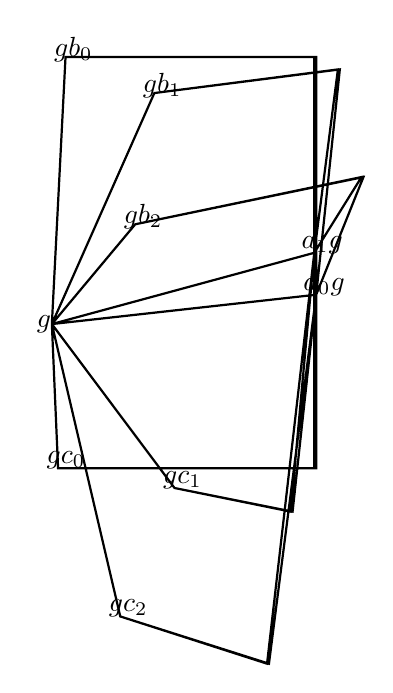
\begin{tikzpicture}
            \draw[thick](0,0)(0,0) -- (0.1733497710540648,3.390812091174084) -- (3.357022945858141,3.390812091174084) -- (3.357022945858141,0.37289587626301607) -- (0,0)
(0,0) -- (1.301722207165342,2.93392954346948) -- (3.6570229458581407,3.23392954346948) -- (3.357022945858141,0.37289587626301607) -- (0,0)
(0,0) -- (1.058935012735694,1.2671696862823545) -- (3.957022945858141,1.8671696862823546) -- (3.357022945858141,0.37289587626301607) -- (0,0)
(0,0) -- (0.1733497710540648,3.390812091174084) -- (3.3326607532801216,3.390812091174084) -- (3.3326607532801216,0.9051238133301255) -- (0,0)
(0,0) -- (1.301722207165342,2.93392954346948) -- (3.6326607532801214,3.23392954346948) -- (3.3326607532801216,0.9051238133301255) -- (0,0)
(0,0) -- (1.058935012735694,1.2671696862823545) -- (3.9326607532801217,1.8671696862823546) -- (3.3326607532801216,0.9051238133301255) -- (0,0)
(0,0) -- (0.07883404051529741,-1.8300862093386594) -- (3.357022945858141,-1.8300862093386594) -- (3.357022945858141,0.37289587626301607) -- (0,0)
(0,0) -- (1.5579215969812215,-2.0820010758898024) -- (3.057022945858141,-2.3820010758898023) -- (3.357022945858141,0.37289587626301607) -- (0,0)
(0,0) -- (0.8685632635483633,-3.7130026232403717) -- (2.757022945858141,-4.313002623240371) -- (3.357022945858141,0.37289587626301607) -- (0,0)
(0,0) -- (0.07883404051529741,-1.8300862093386594) -- (3.3326607532801216,-1.8300862093386594) -- (3.3326607532801216,0.9051238133301255) -- (0,0)
(0,0) -- (1.5579215969812215,-2.0820010758898024) -- (3.0326607532801217,-2.3820010758898023) -- (3.3326607532801216,0.9051238133301255) -- (0,0)
(0,0) -- (0.8685632635483633,-3.7130026232403717) -- (2.7326607532801215,-4.313002623240371) -- (3.3326607532801216,0.9051238133301255) -- (0,0)
;
\node at (-0.1,0) {$ g $};
\node at (3.457022945858141,0.4728958762630161) {$ a_{ 0 }g $};
\node at (3.4326607532801217,1.0051238133301255) {$ a_{ 1 }g $};
\node at (0.27334977105406477,3.4908120911740843) {$ gb_{ 0 } $};
\node at (1.4017222071653421,3.03392954346948) {$ gb_{ 1 } $};
\node at (1.158935012735694,1.3671696862823546) {$ gb_{ 2 } $};
\node at (0.17883404051529742,-1.7300862093386593) {$ gc_{ 0 } $};
\node at (1.6579215969812215,-1.9820010758898023) {$ gc_{ 1 } $};
\node at (0.9685632635483633,-3.6130026232403716) {$ gc_{ 2 } $};

            \end{tikzpicture}
            \end{center}
            \caption{Square of the complex, with edges $(g,ag), (agb, gb) \in E_A,
            (g,gb), (agb, ag) \in E_B.$ \label{fig:square}
            }
            \end{figure}
 \begin{figure}[H]
            %\label{fig:square}
            \begin{center}
            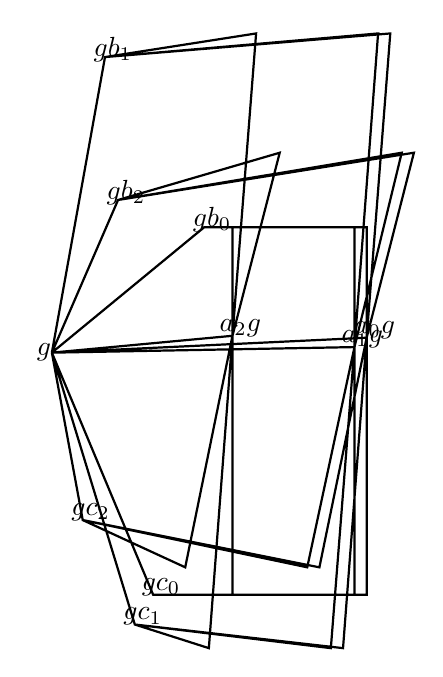
\begin{tikzpicture}
            \draw[thick](0,0)(0,0) -- (1.9342751539770346,1.592146787486484) -- (3.9977159650483194,1.592146787486484) -- (3.9977159650483194,0.1895139068815661) -- (0,0)
(0,0) -- (0.6747529747318886,3.7537814833483254) -- (4.29771596504832,4.053781483348326) -- (3.9977159650483194,0.1895139068815661) -- (0,0)
(0,0) -- (0.8406670989556684,1.9389403650946644) -- (4.5977159650483195,2.5389403650946645) -- (3.9977159650483194,0.1895139068815661) -- (0,0)
(0,0) -- (1.9342751539770346,1.592146787486484) -- (3.8430136066564957,1.592146787486484) -- (3.8430136066564957,0.07060043622967194) -- (0,0)
(0,0) -- (0.6747529747318886,3.7537814833483254) -- (4.1430136066564955,4.053781483348326) -- (3.8430136066564957,0.07060043622967194) -- (0,0)
(0,0) -- (0.8406670989556684,1.9389403650946644) -- (4.443013606656495,2.5389403650946645) -- (3.8430136066564957,0.07060043622967194) -- (0,0)
(0,0) -- (1.9342751539770346,1.592146787486484) -- (2.293632120284654,1.592146787486484) -- (2.293632120284654,0.2139130032702703) -- (0,0)
(0,0) -- (0.6747529747318886,3.7537814833483254) -- (2.5936321202846537,4.053781483348326) -- (2.293632120284654,0.2139130032702703) -- (0,0)
(0,0) -- (0.8406670989556684,1.9389403650946644) -- (2.893632120284654,2.5389403650946645) -- (2.293632120284654,0.2139130032702703) -- (0,0)
(0,0) -- (1.2865857293010516,-3.075251571095318) -- (3.9977159650483194,-3.075251571095318) -- (3.9977159650483194,0.1895139068815661) -- (0,0)
(0,0) -- (1.0536211153180517,-3.4528072818309226) -- (3.6977159650483196,-3.7528072818309224) -- (3.9977159650483194,0.1895139068815661) -- (0,0)
(0,0) -- (0.3921577169609234,-2.126340501500475) -- (3.3977159650483193,-2.726340501500475) -- (3.9977159650483194,0.1895139068815661) -- (0,0)
(0,0) -- (1.2865857293010516,-3.075251571095318) -- (3.8430136066564957,-3.075251571095318) -- (3.8430136066564957,0.07060043622967194) -- (0,0)
(0,0) -- (1.0536211153180517,-3.4528072818309226) -- (3.543013606656496,-3.7528072818309224) -- (3.8430136066564957,0.07060043622967194) -- (0,0)
(0,0) -- (0.3921577169609234,-2.126340501500475) -- (3.2430136066564956,-2.726340501500475) -- (3.8430136066564957,0.07060043622967194) -- (0,0)
(0,0) -- (1.2865857293010516,-3.075251571095318) -- (2.293632120284654,-3.075251571095318) -- (2.293632120284654,0.2139130032702703) -- (0,0)
(0,0) -- (1.0536211153180517,-3.4528072818309226) -- (1.9936321202846539,-3.7528072818309224) -- (2.293632120284654,0.2139130032702703) -- (0,0)
(0,0) -- (0.3921577169609234,-2.126340501500475) -- (1.6936321202846538,-2.726340501500475) -- (2.293632120284654,0.2139130032702703) -- (0,0)
;
\node at (-0.1,0) {$ g $};
\node at (4.0977159650483195,0.2895139068815661) {$ a_{ 0 }g $};
\node at (3.943013606656496,0.17060043622967194) {$ a_{ 1 }g $};
\node at (2.393632120284654,0.3139130032702703) {$ a_{ 2 }g $};
\node at (2.0342751539770347,1.6921467874864842) {$ gb_{ 0 } $};
\node at (0.7747529747318885,3.8537814833483255) {$ gb_{ 1 } $};
\node at (0.9406670989556684,2.0389403650946645) {$ gb_{ 2 } $};
\node at (1.3865857293010517,-2.975251571095318) {$ gc_{ 0 } $};
\node at (1.1536211153180518,-3.3528072818309225) {$ gc_{ 1 } $};
\node at (0.49215771696092336,-2.0263405015004747) {$ gc_{ 2 } $};

            \end{tikzpicture}
            \end{center}
            \caption{Square of the complex, with edges $(g,ag), (agb, gb) \in E_A,
            (g,gb), (agb, ag) \in E_B.$ \label{fig:square}
            }
            \end{figure}
 \begin{figure}[H]
            %\label{fig:square}
            \begin{center}
            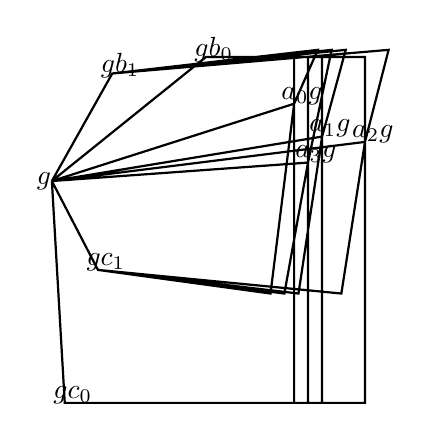
\begin{tikzpicture}
            \draw[thick](0,0)(0,0) -- (1.9557586431264,1.57438884555053) -- (3.0767166665387164,1.57438884555053) -- (3.0767166665387164,0.9819556592155184) -- (0,0)
(0,0) -- (0.7670572145767001,1.3659673224242286) -- (3.3767166665387163,1.6659673224242286) -- (3.0767166665387164,0.9819556592155184) -- (0,0)
(0,0) -- (1.9557586431264,1.57438884555053) -- (3.4319498955442755,1.57438884555053) -- (3.4319498955442755,0.5646741737795121) -- (0,0)
(0,0) -- (0.7670572145767001,1.3659673224242286) -- (3.7319498955442754,1.6659673224242286) -- (3.4319498955442755,0.5646741737795121) -- (0,0)
(0,0) -- (1.9557586431264,1.57438884555053) -- (3.976441748956246,1.57438884555053) -- (3.976441748956246,0.4969328798487971) -- (0,0)
(0,0) -- (0.7670572145767001,1.3659673224242286) -- (4.276441748956246,1.6659673224242286) -- (3.976441748956246,0.4969328798487971) -- (0,0)
(0,0) -- (1.9557586431264,1.57438884555053) -- (3.252869984113015,1.57438884555053) -- (3.252869984113015,0.23445173218235538) -- (0,0)
(0,0) -- (0.7670572145767001,1.3659673224242286) -- (3.552869984113015,1.6659673224242286) -- (3.252869984113015,0.23445173218235538) -- (0,0)
(0,0) -- (0.16369205256408703,-2.8174645610946025) -- (3.0767166665387164,-2.8174645610946025) -- (3.0767166665387164,0.9819556592155184) -- (0,0)
(0,0) -- (0.5853752201947808,-1.1286295443272878) -- (2.7767166665387166,-1.4286295443272878) -- (3.0767166665387164,0.9819556592155184) -- (0,0)
(0,0) -- (0.16369205256408703,-2.8174645610946025) -- (3.4319498955442755,-2.8174645610946025) -- (3.4319498955442755,0.5646741737795121) -- (0,0)
(0,0) -- (0.5853752201947808,-1.1286295443272878) -- (3.1319498955442757,-1.4286295443272878) -- (3.4319498955442755,0.5646741737795121) -- (0,0)
(0,0) -- (0.16369205256408703,-2.8174645610946025) -- (3.976441748956246,-2.8174645610946025) -- (3.976441748956246,0.4969328798487971) -- (0,0)
(0,0) -- (0.5853752201947808,-1.1286295443272878) -- (3.676441748956246,-1.4286295443272878) -- (3.976441748956246,0.4969328798487971) -- (0,0)
(0,0) -- (0.16369205256408703,-2.8174645610946025) -- (3.252869984113015,-2.8174645610946025) -- (3.252869984113015,0.23445173218235538) -- (0,0)
(0,0) -- (0.5853752201947808,-1.1286295443272878) -- (2.9528699841130153,-1.4286295443272878) -- (3.252869984113015,0.23445173218235538) -- (0,0)
;
\node at (-0.1,0) {$ g $};
\node at (3.1767166665387165,1.0819556592155184) {$ a_{ 0 }g $};
\node at (3.5319498955442756,0.6646741737795121) {$ a_{ 1 }g $};
\node at (4.0764417489562454,0.5969328798487971) {$ a_{ 2 }g $};
\node at (3.352869984113015,0.33445173218235535) {$ a_{ 3 }g $};
\node at (2.0557586431264,1.67438884555053) {$ gb_{ 0 } $};
\node at (0.8670572145767,1.4659673224242287) {$ gb_{ 1 } $};
\node at (0.263692052564087,-2.7174645610946024) {$ gc_{ 0 } $};
\node at (0.6853752201947808,-1.0286295443272877) {$ gc_{ 1 } $};

            \end{tikzpicture}
            \end{center}
            \caption{Square of the complex, with edges $(g,ag), (agb, gb) \in E_A,
            (g,gb), (agb, ag) \in E_B.$ \label{fig:square}
            }
            \end{figure}
 \begin{figure}[H]
            %\label{fig:square}
            \begin{center}
            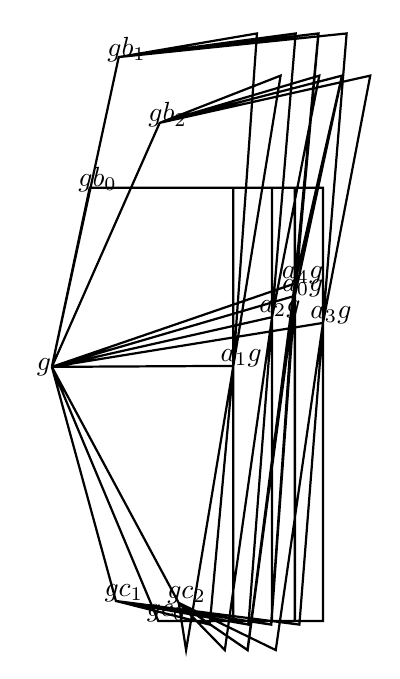
\begin{tikzpicture}
            \draw[thick](0,0)(0,0) -- (0.4805117662300118,2.275705951076729) -- (3.0865232594474152,2.275705951076729) -- (3.0865232594474152,0.9025244499097208) -- (0,0)
(0,0) -- (0.8492429832586497,3.9343137143138502) -- (3.386523259447415,4.23431371431385) -- (3.0865232594474152,0.9025244499097208) -- (0,0)
(0,0) -- (1.3694867810115685,3.0986147891732827) -- (3.6865232594474153,3.698614789173283) -- (3.0865232594474152,0.9025244499097208) -- (0,0)
(0,0) -- (0.4805117662300118,2.275705951076729) -- (2.3047194485279467,2.275705951076729) -- (2.3047194485279467,0.012341930298609593) -- (0,0)
(0,0) -- (0.8492429832586497,3.9343137143138502) -- (2.6047194485279466,4.23431371431385) -- (2.3047194485279467,0.012341930298609593) -- (0,0)
(0,0) -- (1.3694867810115685,3.0986147891732827) -- (2.904719448527947,3.698614789173283) -- (2.3047194485279467,0.012341930298609593) -- (0,0)
(0,0) -- (0.4805117662300118,2.275705951076729) -- (2.796264766558026,2.275705951076729) -- (2.796264766558026,0.6311183473515467) -- (0,0)
(0,0) -- (0.8492429832586497,3.9343137143138502) -- (3.0962647665580256,4.23431371431385) -- (2.796264766558026,0.6311183473515467) -- (0,0)
(0,0) -- (1.3694867810115685,3.0986147891732827) -- (3.396264766558026,3.698614789173283) -- (2.796264766558026,0.6311183473515467) -- (0,0)
(0,0) -- (0.4805117662300118,2.275705951076729) -- (3.4433220197739476,2.275705951076729) -- (3.4433220197739476,0.5583296052668418) -- (0,0)
(0,0) -- (0.8492429832586497,3.9343137143138502) -- (3.7433220197739474,4.23431371431385) -- (3.4433220197739476,0.5583296052668418) -- (0,0)
(0,0) -- (1.3694867810115685,3.0986147891732827) -- (4.043322019773948,3.698614789173283) -- (3.4433220197739476,0.5583296052668418) -- (0,0)
(0,0) -- (0.4805117662300118,2.275705951076729) -- (3.0841571112756583,2.275705951076729) -- (3.0841571112756583,1.0580895850198864) -- (0,0)
(0,0) -- (0.8492429832586497,3.9343137143138502) -- (3.384157111275658,4.23431371431385) -- (3.0841571112756583,1.0580895850198864) -- (0,0)
(0,0) -- (1.3694867810115685,3.0986147891732827) -- (3.6841571112756584,3.698614789173283) -- (3.0841571112756583,1.0580895850198864) -- (0,0)
(0,0) -- (1.3515003906549732,-3.2275026083518092) -- (3.0865232594474152,-3.2275026083518092) -- (3.0865232594474152,0.9025244499097208) -- (0,0)
(0,0) -- (0.8134473878398873,-2.9734762531637626) -- (2.7865232594474154,-3.2734762531637625) -- (3.0865232594474152,0.9025244499097208) -- (0,0)
(0,0) -- (1.6105222218971886,-2.9968240097844405) -- (2.486523259447415,-3.5968240097844406) -- (3.0865232594474152,0.9025244499097208) -- (0,0)
(0,0) -- (1.3515003906549732,-3.2275026083518092) -- (2.3047194485279467,-3.2275026083518092) -- (2.3047194485279467,0.012341930298609593) -- (0,0)
(0,0) -- (0.8134473878398873,-2.9734762531637626) -- (2.004719448527947,-3.2734762531637625) -- (2.3047194485279467,0.012341930298609593) -- (0,0)
(0,0) -- (1.6105222218971886,-2.9968240097844405) -- (1.7047194485279467,-3.5968240097844406) -- (2.3047194485279467,0.012341930298609593) -- (0,0)
(0,0) -- (1.3515003906549732,-3.2275026083518092) -- (2.796264766558026,-3.2275026083518092) -- (2.796264766558026,0.6311183473515467) -- (0,0)
(0,0) -- (0.8134473878398873,-2.9734762531637626) -- (2.496264766558026,-3.2734762531637625) -- (2.796264766558026,0.6311183473515467) -- (0,0)
(0,0) -- (1.6105222218971886,-2.9968240097844405) -- (2.1962647665580257,-3.5968240097844406) -- (2.796264766558026,0.6311183473515467) -- (0,0)
(0,0) -- (1.3515003906549732,-3.2275026083518092) -- (3.4433220197739476,-3.2275026083518092) -- (3.4433220197739476,0.5583296052668418) -- (0,0)
(0,0) -- (0.8134473878398873,-2.9734762531637626) -- (3.1433220197739478,-3.2734762531637625) -- (3.4433220197739476,0.5583296052668418) -- (0,0)
(0,0) -- (1.6105222218971886,-2.9968240097844405) -- (2.8433220197739475,-3.5968240097844406) -- (3.4433220197739476,0.5583296052668418) -- (0,0)
(0,0) -- (1.3515003906549732,-3.2275026083518092) -- (3.0841571112756583,-3.2275026083518092) -- (3.0841571112756583,1.0580895850198864) -- (0,0)
(0,0) -- (0.8134473878398873,-2.9734762531637626) -- (2.7841571112756585,-3.2734762531637625) -- (3.0841571112756583,1.0580895850198864) -- (0,0)
(0,0) -- (1.6105222218971886,-2.9968240097844405) -- (2.484157111275658,-3.5968240097844406) -- (3.0841571112756583,1.0580895850198864) -- (0,0)
;
\node at (-0.1,0) {$ g $};
\node at (3.1865232594474153,1.0025244499097208) {$ a_{ 0 }g $};
\node at (2.404719448527947,0.1123419302986096) {$ a_{ 1 }g $};
\node at (2.896264766558026,0.7311183473515467) {$ a_{ 2 }g $};
\node at (3.5433220197739477,0.6583296052668418) {$ a_{ 3 }g $};
\node at (3.1841571112756584,1.1580895850198865) {$ a_{ 4 }g $};
\node at (0.5805117662300118,2.375705951076729) {$ gb_{ 0 } $};
\node at (0.9492429832586496,4.03431371431385) {$ gb_{ 1 } $};
\node at (1.4694867810115686,3.198614789173283) {$ gb_{ 2 } $};
\node at (1.4515003906549733,-3.127502608351809) {$ gc_{ 0 } $};
\node at (0.9134473878398873,-2.8734762531637625) {$ gc_{ 1 } $};
\node at (1.7105222218971887,-2.8968240097844404) {$ gc_{ 2 } $};

            \end{tikzpicture}
            \end{center}
            \caption{Square of the complex, with edges $(g,ag), (agb, gb) \in E_A,
            (g,gb), (agb, ag) \in E_B.$ \label{fig:square}
            }
            \end{figure}
 \begin{figure}[H]
            %\label{fig:square}
            \begin{center}
            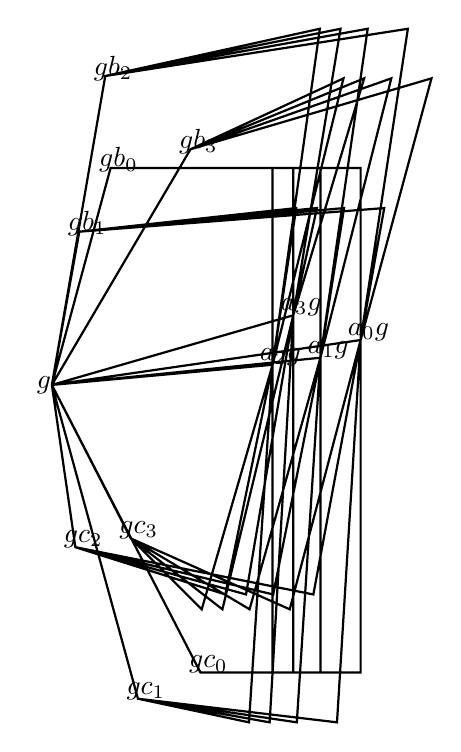
\begin{tikzpicture}
            \draw[thick](0,0)(0,0) -- (0.7458726032165237,2.7557132418413515) -- (3.9209745179927094,2.7557132418413515) -- (3.9209745179927094,0.5699412023352263) -- (0,0)
(0,0) -- (0.3485564412493951,1.9458915209676968) -- (4.220974517992709,2.245891520967697) -- (3.9209745179927094,0.5699412023352263) -- (0,0)
(0,0) -- (0.6779596793098379,3.922871245650283) -- (4.520974517992709,4.522871245650283) -- (3.9209745179927094,0.5699412023352263) -- (0,0)
(0,0) -- (1.7609133057144766,2.993046467574037) -- (4.82097451799271,3.893046467574037) -- (3.9209745179927094,0.5699412023352263) -- (0,0)
(0,0) -- (0.7458726032165237,2.7557132418413515) -- (3.4106911905823374,2.7557132418413515) -- (3.4106911905823374,0.34542895899057785) -- (0,0)
(0,0) -- (0.3485564412493951,1.9458915209676968) -- (3.710691190582337,2.245891520967697) -- (3.4106911905823374,0.34542895899057785) -- (0,0)
(0,0) -- (0.6779596793098379,3.922871245650283) -- (4.010691190582337,4.522871245650283) -- (3.4106911905823374,0.34542895899057785) -- (0,0)
(0,0) -- (1.7609133057144766,2.993046467574037) -- (4.310691190582338,3.893046467574037) -- (3.4106911905823374,0.34542895899057785) -- (0,0)
(0,0) -- (0.7458726032165237,2.7557132418413515) -- (2.8031332529330557,2.7557132418413515) -- (2.8031332529330557,0.2559882534627674) -- (0,0)
(0,0) -- (0.3485564412493951,1.9458915209676968) -- (3.1031332529330555,2.245891520967697) -- (2.8031332529330557,0.2559882534627674) -- (0,0)
(0,0) -- (0.6779596793098379,3.922871245650283) -- (3.403133252933056,4.522871245650283) -- (2.8031332529330557,0.2559882534627674) -- (0,0)
(0,0) -- (1.7609133057144766,2.993046467574037) -- (3.7031332529330556,3.893046467574037) -- (2.8031332529330557,0.2559882534627674) -- (0,0)
(0,0) -- (0.7458726032165237,2.7557132418413515) -- (3.0659012027537775,2.7557132418413515) -- (3.0659012027537775,0.8842645158529634) -- (0,0)
(0,0) -- (0.3485564412493951,1.9458915209676968) -- (3.3659012027537774,2.245891520967697) -- (3.0659012027537775,0.8842645158529634) -- (0,0)
(0,0) -- (0.6779596793098379,3.922871245650283) -- (3.6659012027537776,4.522871245650283) -- (3.0659012027537775,0.8842645158529634) -- (0,0)
(0,0) -- (1.7609133057144766,2.993046467574037) -- (3.9659012027537774,3.893046467574037) -- (3.0659012027537775,0.8842645158529634) -- (0,0)
(0,0) -- (1.8872904584498793,-3.651980756593666) -- (3.9209745179927094,-3.651980756593666) -- (3.9209745179927094,0.5699412023352263) -- (0,0)
(0,0) -- (1.0930977248995042,-3.985239403131553) -- (3.6209745179927095,-4.285239403131553) -- (3.9209745179927094,0.5699412023352263) -- (0,0)
(0,0) -- (0.2985658920612295,-2.0611033209237726) -- (3.3209745179927093,-2.6611033209237727) -- (3.9209745179927094,0.5699412023352263) -- (0,0)
(0,0) -- (1.0019059762683433,-1.9496917534730054) -- (3.0209745179927094,-2.8496917534730053) -- (3.9209745179927094,0.5699412023352263) -- (0,0)
(0,0) -- (1.8872904584498793,-3.651980756593666) -- (3.4106911905823374,-3.651980756593666) -- (3.4106911905823374,0.34542895899057785) -- (0,0)
(0,0) -- (1.0930977248995042,-3.985239403131553) -- (3.1106911905823376,-4.285239403131553) -- (3.4106911905823374,0.34542895899057785) -- (0,0)
(0,0) -- (0.2985658920612295,-2.0611033209237726) -- (2.8106911905823373,-2.6611033209237727) -- (3.4106911905823374,0.34542895899057785) -- (0,0)
(0,0) -- (1.0019059762683433,-1.9496917534730054) -- (2.5106911905823375,-2.8496917534730053) -- (3.4106911905823374,0.34542895899057785) -- (0,0)
(0,0) -- (1.8872904584498793,-3.651980756593666) -- (2.8031332529330557,-3.651980756593666) -- (2.8031332529330557,0.2559882534627674) -- (0,0)
(0,0) -- (1.0930977248995042,-3.985239403131553) -- (2.503133252933056,-4.285239403131553) -- (2.8031332529330557,0.2559882534627674) -- (0,0)
(0,0) -- (0.2985658920612295,-2.0611033209237726) -- (2.2031332529330556,-2.6611033209237727) -- (2.8031332529330557,0.2559882534627674) -- (0,0)
(0,0) -- (1.0019059762683433,-1.9496917534730054) -- (1.9031332529330558,-2.8496917534730053) -- (2.8031332529330557,0.2559882534627674) -- (0,0)
(0,0) -- (1.8872904584498793,-3.651980756593666) -- (3.0659012027537775,-3.651980756593666) -- (3.0659012027537775,0.8842645158529634) -- (0,0)
(0,0) -- (1.0930977248995042,-3.985239403131553) -- (2.7659012027537777,-4.285239403131553) -- (3.0659012027537775,0.8842645158529634) -- (0,0)
(0,0) -- (0.2985658920612295,-2.0611033209237726) -- (2.4659012027537774,-2.6611033209237727) -- (3.0659012027537775,0.8842645158529634) -- (0,0)
(0,0) -- (1.0019059762683433,-1.9496917534730054) -- (2.1659012027537776,-2.8496917534730053) -- (3.0659012027537775,0.8842645158529634) -- (0,0)
;
\node at (-0.1,0) {$ g $};
\node at (4.020974517992709,0.6699412023352262) {$ a_{ 0 }g $};
\node at (3.5106911905823375,0.4454289589905779) {$ a_{ 1 }g $};
\node at (2.903133252933056,0.3559882534627674) {$ a_{ 2 }g $};
\node at (3.1659012027537776,0.9842645158529634) {$ a_{ 3 }g $};
\node at (0.8458726032165237,2.8557132418413516) {$ gb_{ 0 } $};
\node at (0.4485564412493951,2.0458915209676967) {$ gb_{ 1 } $};
\node at (0.7779596793098379,4.022871245650283) {$ gb_{ 2 } $};
\node at (1.8609133057144767,3.093046467574037) {$ gb_{ 3 } $};
\node at (1.9872904584498794,-3.551980756593666) {$ gc_{ 0 } $};
\node at (1.1930977248995043,-3.885239403131553) {$ gc_{ 1 } $};
\node at (0.3985658920612295,-1.9611033209237725) {$ gc_{ 2 } $};
\node at (1.1019059762683434,-1.8496917534730053) {$ gc_{ 3 } $};

            \end{tikzpicture}
            \end{center}
            \caption{Square of the complex, with edges $(g,ag), (agb, gb) \in E_A,
            (g,gb), (agb, ag) \in E_B.$ \label{fig:square}
            }
            \end{figure}
 
\end{multicols*}
  % \printbibliography 
\end{document}

 